
\section{Experimental Setup}\label{sec:expSetup}
This section presents the experimental setup in our platform. We show the datasets in Section~\ref{sec:datasets} and hardware/software setup in Section~\ref{sec:hwswsetup}.

\subsection{Datasets}\label{sec:datasets}
To evaluate our system performance, we employee both real dataset and synthetic dataset.
\subsubsection{Real Dataset}
The real dataset (provided by a commercial large-scale search engine company) consists of two parts: web data and query log. The web data contains more than 10 million web documents. The query log contains around 1 million real queries\footnote{\small The data source as well as more detailed statistics is omitted for a double-blind review.}.

\subsubsection{Synthetic Dataset}
%The synthetic dataset allows us to vary many performance-critical parameters to understand the cases that Smart SSD wins.
The synthetic dataset allows us to better understand various performance-critical parameters in Smart SSDs.
We explain the parameters and the methodology to generate data.
Unless otherwise stated, when varying one parameter, we fix all the rest parameters as defaults.

%Unless otherwise stated, we explain the parameters with two inverted lists, and when varying one particular parameter, we fix all the rest parameters as defaults.


\textbf{Number of lists}. By default, we evaluate the list operations with two inverted lists: list \emph{A} and list \emph{B}. To capture the real case that the list sizes are skewed (i.e., one list is longer than the other), list $A$ represents the shorter list while list $B$ the longer one in this paper unless otherwise stated.
%As we explained later, the size ratio between list $A$ and $B$ is determined by the \emph{skewness factor}.
When varying the number of lists according to a parameter $m$ ($m>1$), we generate $m$ lists independently. Among them, half of the lists ($\lceil m/2\rceil$) are of the same size with list $A$ (i.e., shorter lists), the other half ($\lfloor m/2\rfloor$) are of the same size with list $B$ (i.e., longer lists). We vary the number of lists from 2 to 8.

\textbf{List size skewness factor}. The \emph{skewness factor} is defined as the ratio of the size of the longer list to the that of the shorter list (i.e., $\frac{|B|}{|A|}$). In practice, different lists significantly differ in their sizes because some query terms can be even more popular than the others. We set the skewness factor to 100 by default and vary the skewness factor from 1 to 10,000 to capture the real case\footnote{\small We randomly pick up 10,000 queries from the real query log and run them with the real web data. The average skewness factor is 3672. Even if we remove the top 20\% highest ones, it is still 75.}.

\textbf{Intersection ratio}. The intersection ratio is defined as the intersection size over the shorter list (i.e., $\frac{|A\cap B|}{|A|}$) for two lists $A$ and $B$. By default, we set it to 1\% to reflect the real scenario. E.g., based on Bing search, for 76\% of the queries, the intersection size is two orders of magnitude smaller than the shortest inverted list~\cite{Ding2011}. We vary the intersection ratio from 1\% to 100\%.


\textbf{List size}. Unless otherwise stated, the list size represents the size of the \emph{longer} list (i.e., list \emph{B}).
By default, we set the size of list $B$ to 10 MB, and vary from 1 MB to 100 MB. In real search engines, although the entire inverted index is huge, there are also a huge number of terms with relatively shorter inverted lists (on average, 10s of MBs). The size of list $A$ can be obtained with the skewness factor. Once the list size is determined, we randomly generate a list of entries (each includes the document ID, score, and positions) from a universe~\cite{Ding2011}.


Table~\ref{tab:synData} shows a summary of the key parameters with defaults highlighted in bold.

\begin{table}[tbp]
\centering\small
\begin{tabular}{l|l}\hline\hline
\textbf{Parameters}  &   \textbf{Ranges}   \\\hline
Number of lists & \textbf{2}, 3, 4, 5, 6, 7, 8\\\hline
List size skewness factor  & 10000, 1000, \textbf{100}, 10, 1\\\hline
Intersection ratio  &   0.1\%, \textbf{1\%}, 10\%, 100\%\\\hline
List size & 1 MB, \textbf{10 MB}, 50 MB, 100 MB\\\hline\hline
\end{tabular}
\caption{Parameter setup}\label{tab:synData}
\end{table}



\subsection{Hardware and Software Setup}\label{sec:hwswsetup}
In our experiments, the host machine is a commodity server with Intel i7 processor (3.40 GHz) and 8 GB memory running Windows 7.
The Smart SSD is a size of 400 GB SAS SSD (SLC) and connected to the host machine via a host bus adaptor (HBA) with 6Gbps. The regular SSD is an identical SSD without implementation of query offloading.

We adopt the C++ version (instead of Java version) of Lucene\footnote{\small\url{http://clucene.sourceforge.net}} to be compatible with programming interface of Smart SSDs. We choose the stable 0.9.21 version.

We measure the power consumption via \emph{WattsUp}\footnote{\small \url{https://www.wattsupmeters.com}} as follows. Let $W_1$ and $W_2$ be the power (in Watts) when the system is sufficiently stabilized (i.e., idle) and running, and $t$ be the query latency, the energy is calculated by $(W_2-W_1)\times t$.


%================ Need to proofread from this ======================


\section{Experimental Results}\label{sec:expResults}
In this section, we present our experimental results and analysis of offloading different query operations to Smart SSD: \textsf{intersection} (Section~\ref{sec:expIntersection}), \textsf{ranked intersection} (Section~\ref{sec:expRankedIntersection}),
\textsf{difference} (Section~\ref{sec:expDifference}), \textsf{ranked difference} (Section~\ref{sec:expRankedDifference}), and \textsf{ranked union} (Section~\ref{sec:expRankedUnion}).

We compare two approaches: (1) \emph{Smart SSD}: our integrated Lucene with Smart SSD; (2) \emph{Regular SSD}: the original Lucene on a regular SSD. As our performance metrics, we adopt the average query latency\footnote{\small Due to the current limitation of the Smart SSD (it can only support one concurrent request each time), we measure the query latency instead of the query throughput. This limitation will be resolved in the next-generation of Smart SSDs.} and energy consumption.

%As explained in Section~\ref{sec:implementation}, we improved the original Lucene implementations on some list operations (e.g., intersection). Thus, we compare the following three approaches. (1) \emph{Smart SSD}: run our integrated Lucene and Smart SSD; (2) \emph{Regular SSD}: run the original Lucene on a regular SSD; (3) \emph{Regular SSD (optimized)}: run our optimized Lucene on a regular SSD.

%We measure the average query latency and energy consumption. %We may also report the normalized values~\cite{Ding2011}.

\subsection{Intersection}\label{sec:expIntersection}
In this case, we offload the \textsf{intersection} to Smart SSD. That is, step S3 and S4 are executed inside SSD.

\textbf{Results on real data}.
Table~\ref{tab:interRealData} shows the averaged query latency and energy consumption with a reply of the real queries on the real web data. It clearly shows that, compared to regular SSD, Smart SSD can reduce query latency by 2.2$\times$ and energy by 6.7$\times$. The performance gain of the query latency comes from the high internal bandwidth and low I/O latency of Smart SSD. In addition, the energy saving results from less data movement and the power-efficient processors inside SSD.

\begin{table}[tbp]\small
\centering
\begin{tabular}{l|c|c}\hline\hline
& \textbf{Query latency (ms)} & \textbf{Energy (mJ)}\\\hline
Smart SSD & 97 & 204\\\hline
Regular SSD & 210 & 1365 \\\hline\hline
\end{tabular}
\caption{Intersection on real data}\label{tab:interRealData}
\end{table}

For more detailed analysis, we chose a particular query with two query terms. Let $A$ and $B$ be the inverted lists of the two terms, where the number of entries in $A$ and $B$ are 2,938 and 65,057 respectively. Figure~\ref{fig:timeBreakDownRegSmart} shows the time breakdown of running Lucene on the regular SSD and the Smart SSD. It illustrates that Smart SSD can reduce the I/O time from 54.8 ms to	14.5 ms (i.e., a factor of 3.8). This is the speedup upper bound that Smart SSD can achieve. However, Smart SSD also increase the CPU time from 8 ms to 16.6 ms. Consequently, Smart SSDs can overall achieve around 2$\times$ speedup in query latency.

\begin{figure}[tbp]
%\vspace{-5mm}
	\centering
		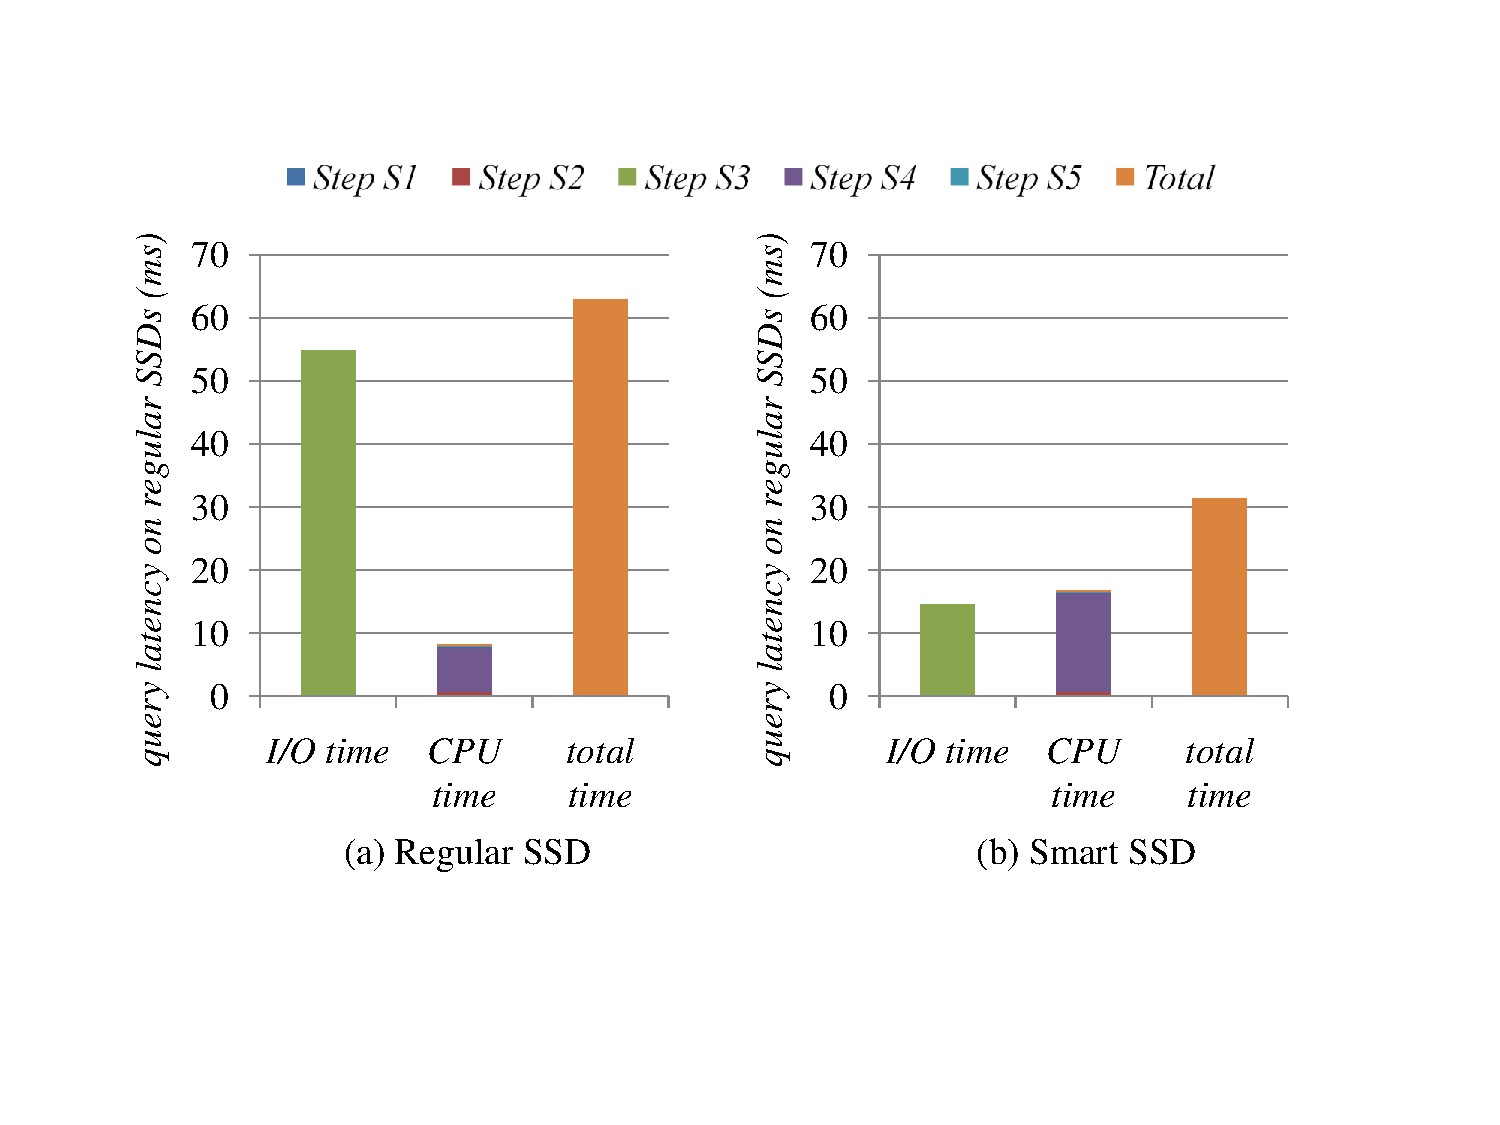
\includegraphics[width=1\columnwidth]{figures/timeBreakDownRegSmart.pdf}
	\caption{\small Query latency breakdown of Lucene running on the regular SSD and the Smart SSD, for a particular real query.}
	\label{fig:timeBreakDownRegSmart}
\end{figure}

Now, we break further down the time for the query processing only inside Smart SSDs. We consider step S3 and S4 since other steps are executed at the host side and the time is ignorable (please see CPU time in Figure~\ref{fig:timeBreakDownRegSmart}).
As shown in Figure~\ref{fig:timeBreakDownSmartSSD}, loading inverted lists from flash chips to the device DRAM (Load data) is still a dominant bottleneck (48\%), which can be alleviated by increasing the internal bandwidth. The next bottleneck (28\%) is memory access (Memcpy), which can be mitigated by reducing memory access cost (e.g., using DMA copy or more caches). Processor speed (Intersection) is the next bottleneck (22\%). This can be reduced by adopting more powerful processors. However, balance over bus architecture, memory technology, and CPU architecture for SSD system is also important.

\begin{figure}[tbp]
	\centering
		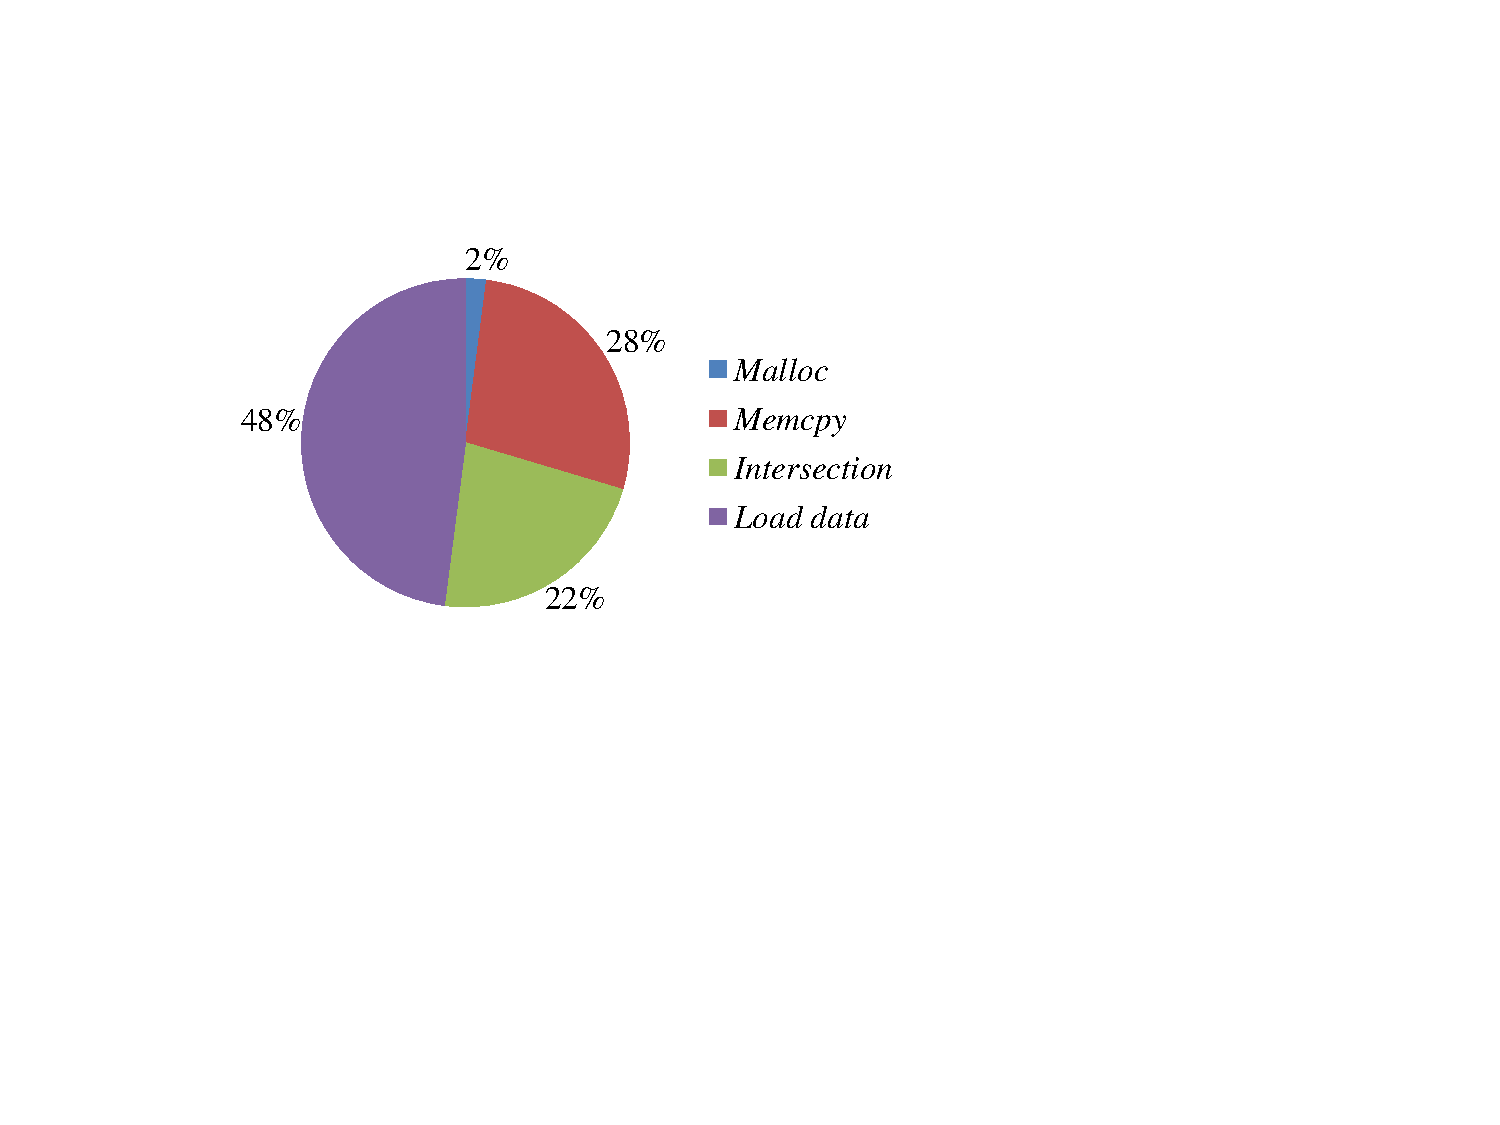
\includegraphics[width=0.7\columnwidth]{figures/timeBreakDownSmartSSD.pdf}
	\caption{\small Time breakdown of executing list intersection on Smart SSDs}
	\label{fig:timeBreakDownSmartSSD}
\end{figure}


\textbf{Effect of varying list size}.
Figure~\ref{fig:varyListSizeIntersection} displays the effect of list size which affects the I/O time (that is, longer lists imply more I/O time).
We vary the size of list $B$ from 1 MB to 100 MB (while the size of list $A$ depends on the skewness factor whose default value is 100).
Both query latency and energy consumption increase with longer lists because of more I/Os.
On average, Smart SSD reduces query latency by a factor of 2.5 and energy by a factor of 7.8 compared to regular SSD.
Figure ~\ref{fig:varyListSizeIntersection} delivers the following implication: \emph{Smart SSD favors longer lists for the \textsf{intersection} operation}.

\begin{figure}[tbp]
  \centering
    \begin{tabular}{ccc}
 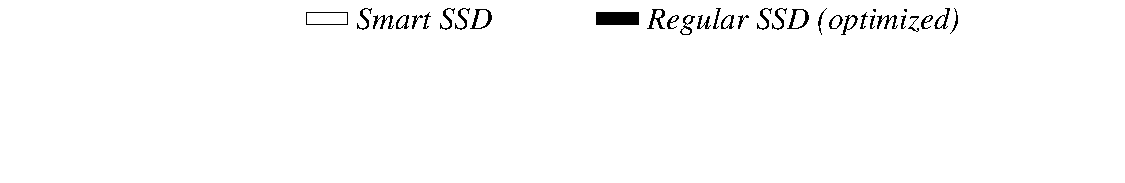
\includegraphics[width=0.52\columnwidth]{figures/banner2.pdf}
\end{tabular}
\vspace{-0.1cm}
\renewcommand{\tabcolsep}{0.1mm}
  \begin{tabular}{ccc}
 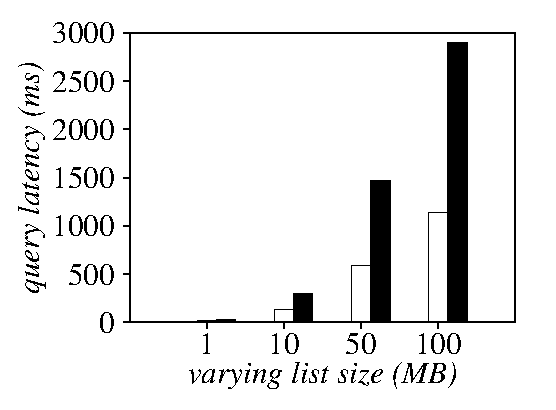
\includegraphics[width=0.5\columnwidth]{figures/Intersection-time-VaryListLen.eps}&
  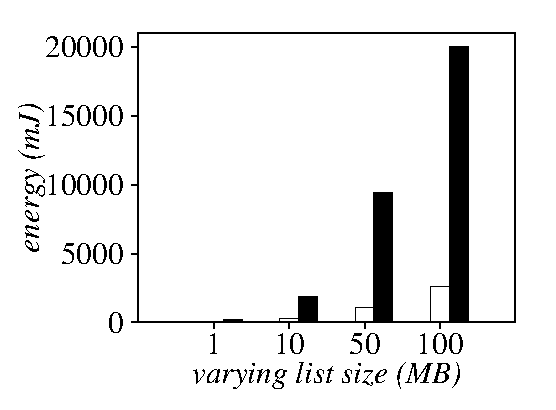
\includegraphics[width=0.5\columnwidth]{figures/Intersection-energy-VaryListLen.eps}\\
  (a) query latency & (b) energy
\end{tabular}
  \caption{Varying the list size (for intersection)}
  \label{fig:varyListSizeIntersection}
 \end{figure}
 


\textbf{Effect of varying list size skewness factor}.
Figure~\ref{fig:varyListSkewIntersection} shows the impact of list size skewness factor $f$, which can affect the adaptive intersection algorithm.
Higher skewness provides more opportunities for skipping data. This favors Smart SSD with less memory access since the memory access inside Smart SSD is expensive.
We vary different skewness factors from 1 to 1000 (while fixing the size of list $B$ to 10 MB). The query latency (as well as energy) drops when $f$ gets higher because the size of list $A$ gets smaller. In any case, Smart SSD outperforms regular SSD significantly in both latency and energy.
Figure~\ref{fig:varyListSkewIntersection} implies: \emph{Smart SSD favors lists with a higher skewness factor for the \textsf{intersection} operation}.

\begin{figure}[tbp]
  \centering
    \begin{tabular}{ccc}
 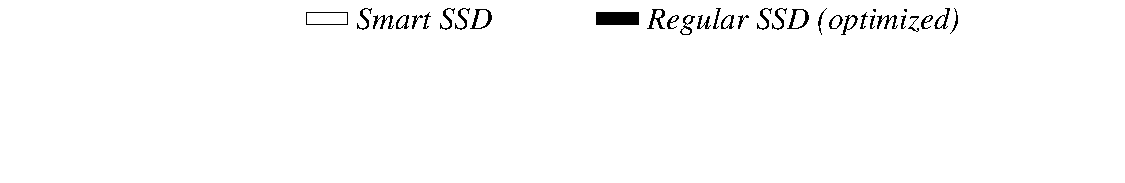
\includegraphics[width=0.52\columnwidth]{figures/banner2.pdf}%banner2.pdf
\end{tabular}
\vspace{-0.1cm}
\renewcommand{\tabcolsep}{0.1mm}


  \begin{tabular}{ccc}
 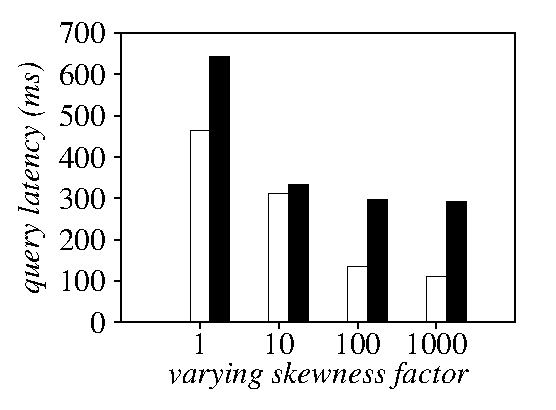
\includegraphics[width=0.5\columnwidth]{figures/Intersection-time-VaryListSkew2.eps}&
  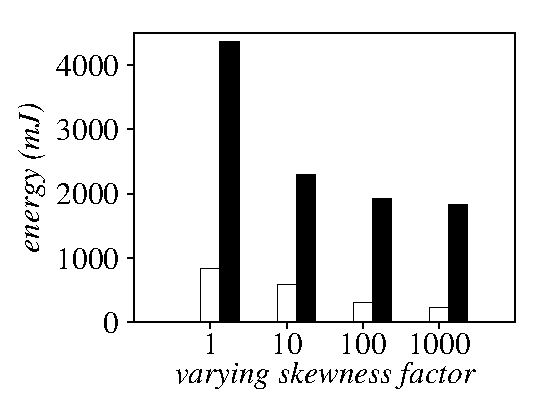
\includegraphics[width=0.5\columnwidth]{figures/Intersection-energy-VaryListSkew2.eps}\\
  (a) query latency & (b) energy\\
\end{tabular}

  \caption{Varying the list size skewness factor (for intersection)}
  \label{fig:varyListSkewIntersection}
 \end{figure}


Besides the superiority of Smart SSD shown in Figure~\ref{fig:varyListSkewIntersection}, it is also interesting to see that the performance gain of the latency in Smart SSD is smallest at $f=10$, not at $f=1$. That is because the \underline{a}verage \underline{n}umber of \underline{m}emory accesses per \underline{p}age (ANMP) is larger than all the other cases at $f=10$ (please see Table \ref{tab:varyListSkewIntersection}). Note that when $f=1$, the sort-merge algorithm is adopted, while the adaptive intersection algorithm is used for all the other cases(as explained in Section \ref{sec:intersection}).

\begin{table}[tbp]\small
\centering
\begin{tabular}{l|l|l|l|l|l}\hline\hline
$f$ & $n_1$ & $n_2$ & $n_p$ & estimated ANMP & real ANMP \\\hline
$1$ & $327680$ & $327680$ & $2564$ & $\frac{n_1+n_2}{n_p}=256$ & $383$ \\\hline
$10$ & $32768$ & $327680$ & $1408$ & $\frac{n_1\cdot\log n_2}{n_p}=427$ & $640$ \\\hline
$100$ & $3277$ & $327680$ & $1284$ & $\frac{n_1\cdot\log n_2}{n_p}=47$ & $68$ \\\hline
$1000$ & $328$ & $327680$ & $1280$ & $\frac{n_1\cdot\log n_2}{n_p}=5$ & $6$ \\\hline\hline
\end{tabular}
\caption{The average number of memory accesses per page (ANMP) in Figure~\ref{fig:varyListSkewIntersection}, where $f$ means the skewness factor, $n_1$ and $n_2$ indicate the number of entries in list $A$ and $B$, $n_p$ is the total number of pages. Note that each page is 8 KB and each entry takes 32 bytes. Thus, each page can contain 256 entries.}\label{tab:varyListSkewIntersection}
\end{table}


\textbf{Effect of varying intersection ratio}.
Figure~\ref{fig:varyInterRatioIntersection1} illustrates the impact of intersection ratio $r$.
It determines the result size which can have an impact on system performance in two aspects: (1) data movement via the host I/O interface; and (2) ranking cost at the host side (since all the qualified document IDs in the result set will be evaluated for ranking). Surprisingly, we cannot find a clear correlation between performance and intersection ratios (please refer to Figure~\ref{fig:varyInterRatioIntersection1}).
That is because, by default, list $A$ includes around 3277 entries (0.1 MB) while list $B$ includes around 327680 entries (10 MB). Even when $r$ is 100\%, the result size is at most 3277. This does not make much difference in both I/O time (around 1.4 ms) and ranking cost (around 0.5 ms).

%Figure~\ref{fig:varyInterRatioIntersection1} shows impact of intersection ratio in the default case. Surprisingly, it does not show a clear impact. The reason is that, the skewness factor is 100, i.e., the size of list $A$ is 1\% smaller than list $B$. In this case, the maximum result size is 3367 (where the intersection ratio is 100\%), i.e., (3367 * 16bytes)/8KB = 7 pages = 1.4 ms, while the ranking cost is around 0.5 ms.




\begin{figure}[tbp]
\centering
\begin{tabular}{ccc}
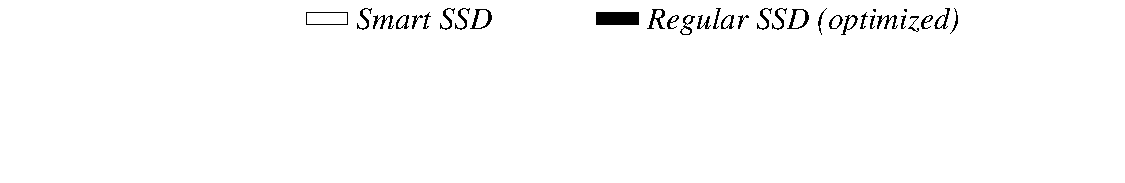
\includegraphics[width=0.52\columnwidth]{figures/banner2.pdf}
\end{tabular}
\vspace{-0.1cm}
\renewcommand{\tabcolsep}{0.1mm}
\begin{tabular}{ccc}
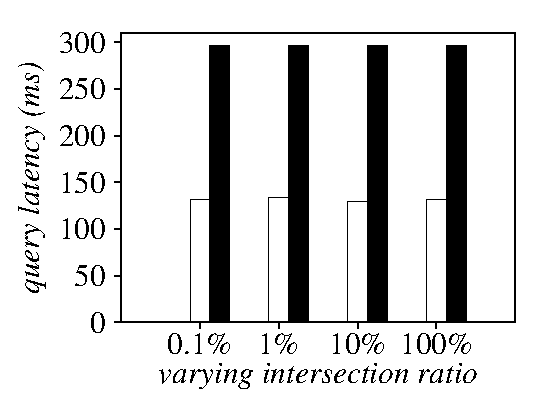
\includegraphics[width=0.5\columnwidth]{figures/Intersection-time-VaryInterRatio.eps}&
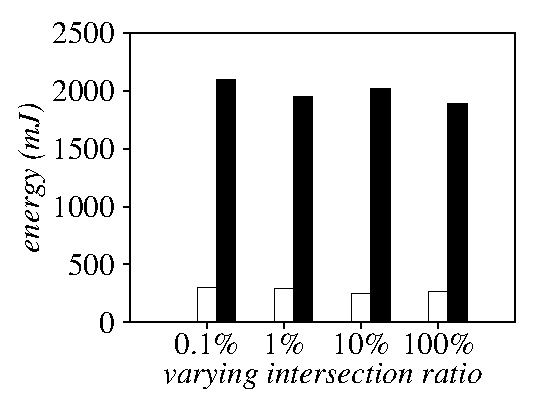
\includegraphics[width=0.5\columnwidth]{figures/Intersection-energy-VaryInterRatio.eps}\\
(a) query latency & (b) energy
\end{tabular}
\caption{Varying intersection ratio (for intersection)}
\label{fig:varyInterRatioIntersection1}
\end{figure}




  \begin{figure}[tbp]
  \centering
    \begin{tabular}{ccc}
 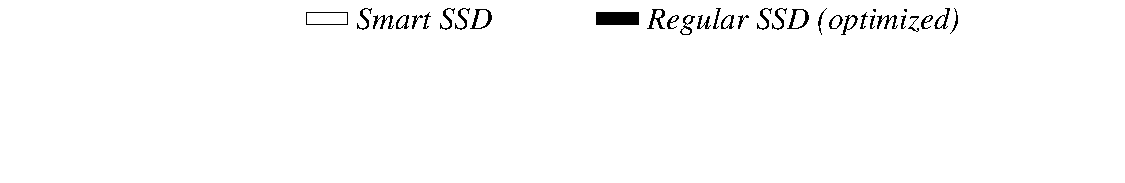
\includegraphics[width=0.52\columnwidth]{figures/banner2.pdf}
\end{tabular}
\vspace{-0.1cm}
\renewcommand{\tabcolsep}{0.1mm}
  \begin{tabular}{ccc}
 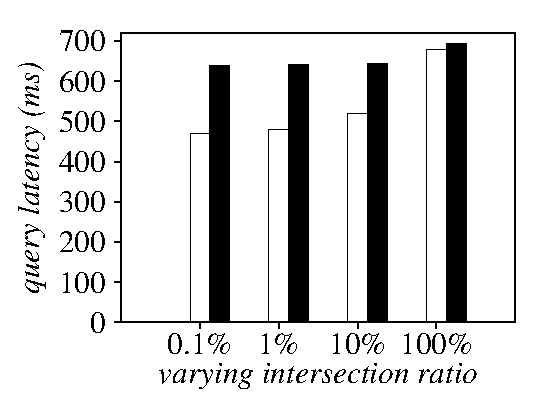
\includegraphics[width=0.5\columnwidth]{figures/Intersection-time-VaryInterRatio-equal2.eps}&
  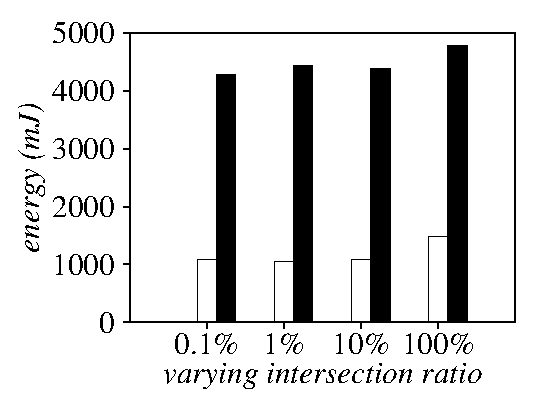
\includegraphics[width=0.5\columnwidth]{figures/Intersection-energy-VaryInterRatio-equal2.eps}\\
  (a) query latency & (b) energy\\
\end{tabular}
  \caption{Varying intersection ratio on equal-sized lists (for intersection)}
  \label{fig:varyInterRatioIntersection2}
 \end{figure}


To verify this result, we make another experiment by setting the size of list $A$ to the same as $B$ (i.e., both are of 10 MB). %The sizes are statistically the same, listA is 327668, listB is 327934, at 100\%, the intersection is 326918.
We see a clear impact of intersection ratio $r$ in the Figure~\ref{fig:varyInterRatioIntersection2}.
Both query latency and energy consumption increase as $r$ gets higher. Particularly when $r$ grows from 10\% to 100\% (the corresponding result size jumps from 32,768 to 327,680), we can see noticeable increase of them. For regular SSD, this increase originates from more ranking cost overhead. For Smart SSD, it results from both data transfer and ranking cost overhead.
In all cases, even when $r$ is 100\%, Smart SSD shows a better performance than regular SSD. That is because, in this case ($r$ is 100\%), Smart SSD only needs to transfer one list, which saves around 50\% of data transfer.
In short, Figure~\ref{fig:varyInterRatioIntersection2} delivers a message: \emph{Smart SSD favors lists with a smaller intersection ratio for the \textsf{intersection} operation}.



%For optimized regular SSD, the increase is because of the extra ranking cost. E.g., from 10\% to 100\%, the optimized regular SSD approach increase around 50 ms, because of dramatic intersection size increase from 32531 to 326918. For Smart SSD, the increase is because of two factors: more data transfer and ranking cost (at the host side). From 10\% to 100\%, the latency increased 163 ms. In which, data transfer increases around 110 ms (((326918 - 32531) * 16 / 8KB) * 0.2 = 115 ms), while the ranking cost increases around 50 ms, same as optimized regular SSD.



%It is also interesting to see in Figure~\ref{fig:varyInterRatioIntersection2}, even when the intersection ratio is 100\%, Smart SSD can still win a bit over optimized regular SSD. That is because, in this case, Smart SSD only needs to transfer one list, saving around 50\% of data transfer.


%Besides that, it is also interesting to see that there is a latency jump between the intersection ratio 10\% and 100\% (Figure~\ref{fig:varyInterRatioIntersection2}(c)).  on regular SSD (lucene version): also a huge increase from 10\% to 100\% (around 2000 ms increase), one reason is because of ranking cost (800 ms more than 10\%), another reason is overhead in ConjunctionScorer::doNext(), where ``flag = more and first().doc smaller than last.doc()", taking around 1000 ms, because of more calls to doNext(), as cannot skip.


\textbf{Effect of varying number of lists}.
Figure~\ref{fig:varyNumKeywordsIntersection} shows the results on the impact of varying the number of lists (i.e., number of terms in a query). %More lists means more I/O time, which Smart SSD can reduce.
We vary the number of lists from 2 to 8.
The query latency (as well as energy) grows with higher number of lists\footnote{\small When the number of lists $u$ goes from 2 to 3, the latency does not increase so much. That is because the generated lists are $\{A, B\}$ and $\{A, B, A\}$ when $u$ is 2 and 3, respectively. Since list $A$ is 100$\times$ smaller than list $B$, thus, it does not incur much overhead in query latency.} because of more data transfer.
On average, Smart SSD reduces query latency by 2.6$\times$ and energy by 9.5$\times$.
In short, Figure~\ref{fig:varyNumKeywordsIntersection} delivers a message: \emph{Smart SSD favors more lists for the \textsf{intersection} operation}.

  \begin{figure}[htbp]
  \centering
    \begin{tabular}{ccc}
 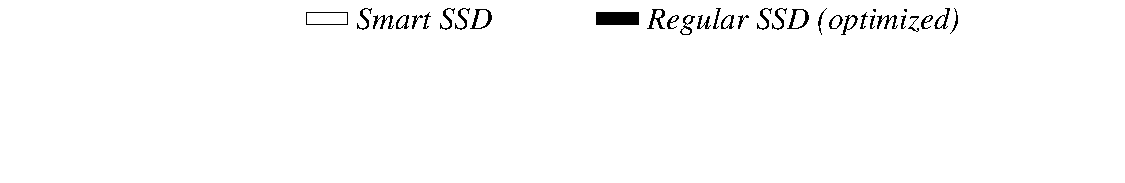
\includegraphics[width=0.52\columnwidth]{figures/banner2.pdf}
\end{tabular}
\vspace{-0.1cm}
\renewcommand{\tabcolsep}{0.1mm}
  \begin{tabular}{ccc}
 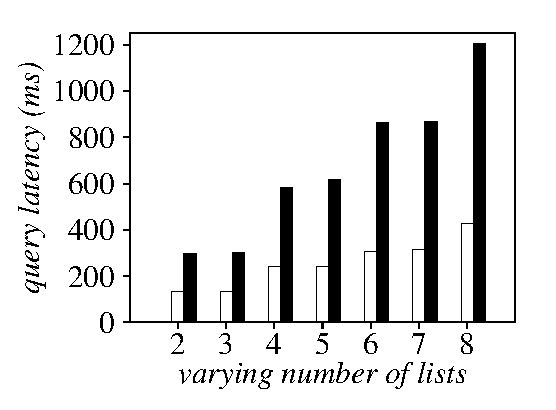
\includegraphics[width=0.5\columnwidth]{figures/Intersection-time-VaryNumLists.eps}&
  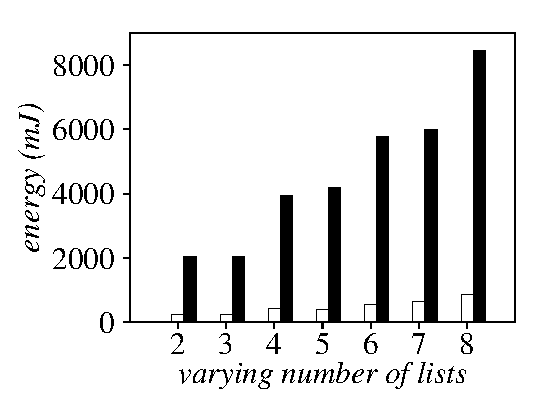
\includegraphics[width=0.5\columnwidth]{figures/Intersection-energy-VaryNumLists.eps}\\
  (a) query latency & (b) energy
\end{tabular}
  \caption{Varying the number of lists (for intersection)}
  \label{fig:varyNumKeywordsIntersection}
 \end{figure}

\textbf{Remark}. The \textsf{intersection} operation can be cost-effectively offloaded to Smart SSD, especially when the number of lists is high, the lists are long, the list sizes are skewed, and the intersection ratio is low.

\subsection{Ranked Intersection}\label{sec:expRankedIntersection}
In this case, we offload the \textsf{ranked intersection} (i.e., step S3, S4, and S5 in Figure~\ref{fig:SmartSSDLucene}) to Smart SSD. Compared to the offloading of intersection-only operation (Section~\ref{sec:expIntersection}), offloading ranked intersection can (1) save data transfer since only the top ranked results are returned; but (2) increase the cost of ranking inside the device. However, there is not much difference when the result size is small (e.g., less than 30,000 entries). As a reference, sending back 30,000 entries from Smart SSD to the host takes around 12 ms, and ranking 30,000 entries at host side takes around 5 ms (Figure \protect\ref{fig:varyInterRatioIntersection2}).

\textbf{Results on real data}.
The results are similar to the non-ranked version(see Table~\ref{tab:interRealData}). So, we omit them due to space limitations. Since the average intersection result size is 1,144, it will not make a significant difference (less than 1 ms).


%Table~\ref{tab:rankInterRealData} shows the results by a replay of the real queries on the real web data. It shows that, Smart SSD  can reduce the query latency by 2.2$\times$ and energy by 7.8$\times$ compared to regular SSD. The results are largely similar to the non-ranked intersection (see Table~\ref{tab:interRealData}). That is because the average intersection result size is 1144, which will not make a significant difference (less than 1 ms).

%\begin{table}[tbp]\small
%\centering
%\begin{tabular}{l|c|c}\hline\hline
%& \textbf{Query latency (ms)} & \textbf{Energy (mJ)}\\\hline
%Smart SSD & 96 & 183\\\hline
%Regular SSD & 210 & 1428 \\\hline\hline
%\end{tabular}
%\caption{Ranked intersection on real data \textcolor{red}{omit}}\label{tab:rankInterRealData}
%\end{table}

\textbf{Effect of varying list size}.
The results of varying list size are also similar to non-ranked intersection (i.e., Figure~\ref{fig:varyListSizeIntersection}) because the intersection size is small. As an example, the maximum intersection size is 359 (when the list size is 100 MB) and the minimum intersection size is 3 (when the list size is 1 MB).

\textbf{Effect of varying list size skewness factor}.
The results are similar to the non-ranked version (i.e., Figure~\ref{fig:varyListSkewIntersection}) because the intersection size is not that large. E.g., the maximum intersection size is 3,877 (when the skewness factor is 1). Again, Smart SSD shows a better performance.

\textbf{Effect of varying intersection ratio}.
The results of the default case (i.e., list $A$ is 100$\times$ smaller than list $B$) is similar to Figure~\ref{fig:varyInterRatioIntersection1}, where Smart SSD outperforms regular SSD significantly.

Next, we make another experiment by setting the size of list $A$ to the same as list $B$ (both are 10 MB). Please see Figure~\ref{fig:varyRankInterRatioIntersection2}. High intersection ratio leads to high intersection result size, while causing more overhead for ranking. We vary the intersection ratio from 0.1\% too 100\%.
The query latency (as well as energy consumption) goes up as an intersection ratio increases. However, we cannot see noticeable increase of them compared to the results in Figure~\ref{fig:varyInterRatioIntersection2} for non-ranked intersection offloading. As an example, for Smart SSD, when the intersection ratio changes from 10\% to 100\%, the latency increases by 65 ms in Figure~\ref{fig:varyRankInterRatioIntersection2}, while the corresponding increase in Figure~\ref{fig:varyInterRatioIntersection2} is 163 ms. 
This difference is closely related to the extra data movement. For ranked intersection offloading, since only top-$k$ results are returned, less amount of data needs to move. Please see the query latency at 100\% intersection ratio in both Figure~\ref{fig:varyInterRatioIntersection2} and Figure~\ref{fig:varyRankInterRatioIntersection2}. This demonstrates well our analysis.

%The increase does not go that much is because of no extra data movement (only top-$k$ results are returned), i.e., the increase is owing to the extra ranking cost.

%It is also interesting to see from Figure~\ref{fig:varyRankInterRatioIntersection2} that, when the intersection ratio is 100\%, Smart SSD wins much more than the non-ranked version (Figure~\ref{fig:varyInterRatioIntersection2}). That is because of much less data movement as only top-$k$ results are returned.


  \begin{figure}[tbp]
  \centering
    \begin{tabular}{ccc}
 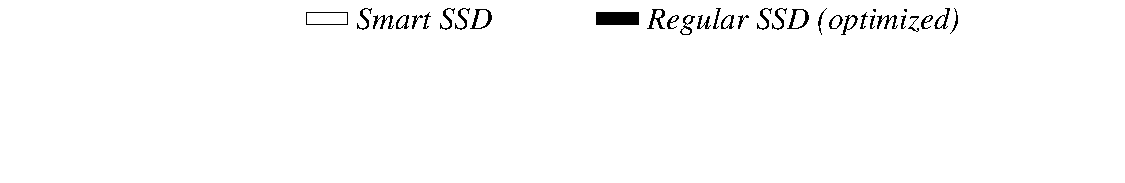
\includegraphics[width=0.52\columnwidth]{figures/banner2.pdf}
\end{tabular}
\vspace{-0.1cm}
\renewcommand{\tabcolsep}{0.1mm}
  \begin{tabular}{ccc}
 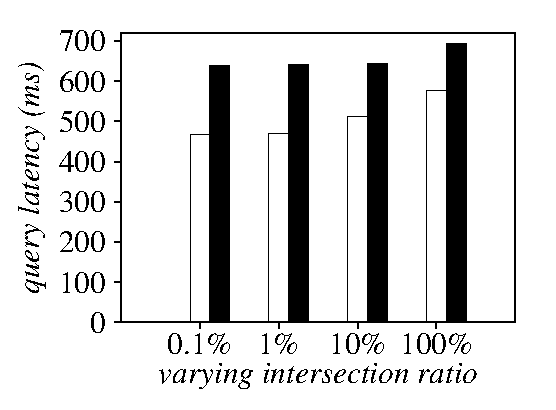
\includegraphics[width=0.5\columnwidth]{figures/RankIntersection-time-VaryInterRatio-equal2.eps}&
  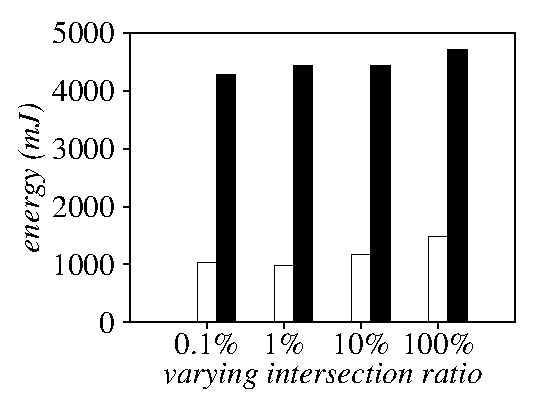
\includegraphics[width=0.5\columnwidth]{figures/RankIntersection-energy-VaryInterRatio-equal2.eps}\\
  (a) query latency & (b) energy\\
\end{tabular}
  \caption{Varying intersection ratio on equal-sized lists (for ranked intersection)}
  \label{fig:varyRankInterRatioIntersection2}
 \end{figure}


\textbf{Effect of varying number of lists}.
The results are similar to the non-ranked version shown in Figure~\ref{fig:varyNumKeywordsIntersection} because the intersection size is very small (only 47), which will not make a major difference.

\subsection{Difference}\label{sec:expDifference}

We offload the \textsf{difference} operation (i.e., step S3 and S4 in Figure~\ref{fig:SmartSSDLucene}) to Smart SSD, and the ranking is executed at the host side. When the \textsf{difference} operator is applied to two lists, it can be $(A-B)$ or $(B-A)$, where the list $A$ is shorter than list $B$. As discussed in Section~\ref{sec:designSpace}, only the former case can potentially benefit from Smart SSD.



\textbf{Results on real data}.
Table~\ref{tab:diffRealData} shows the results with the real queries on the real web data. For each query, we consider the $(A-B)$ case, where $A$ and $B$ indicate the shortest and longest list in a query respectively. It clearly shows that, compared to regular SSD, Smart SSD can achieve better performance: the query latency by 2.5$\times$ and energy consumption by 8.5$\times$.

\begin{table}[tbp]\small
\centering
\begin{tabular}{l|c|c}\hline\hline
& \textbf{Query latency (ms)} & \textbf{Energy (mJ)}\\\hline
Smart SSD & 78 & 148\\\hline
Regular SSD & 194 & 1261 \\\hline\hline
\end{tabular}
\caption{Difference on real data}\label{tab:diffRealData}
\end{table}

\textbf{Effect of varying list size}.
Figure~\ref{fig:varyListSizeDifference} plots the effect of varying list sizes, which affects the I/O time.
We vary the list sizes of list $B$ from 1 MB to 100 MB (while the size of list $A$ depends on the skewness factor).
The query latency (as well as energy consumption) goes up with longer lists.
On average, Smart SSD reduces query latency by 2.7$\times$, and energy consumption by 9.7$\times$.
Figure~\ref{fig:varyListSizeDifference} delivers a message: \emph{Smart SSD favors longer lists for the \textsf{difference} operation}.

\begin{figure}[hbtp]
  \centering
    \begin{tabular}{ccc}
 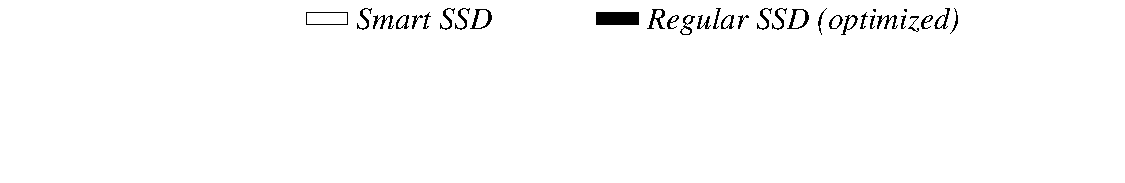
\includegraphics[width=0.52\columnwidth]{figures/banner2.pdf}
\end{tabular}
\vspace{-0.1cm}
\renewcommand{\tabcolsep}{0.1mm}
  \begin{tabular}{ccc}
 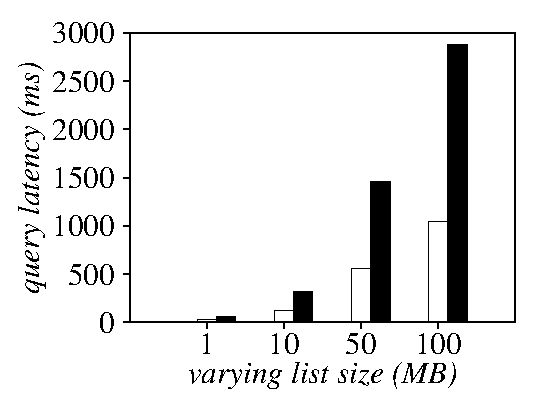
\includegraphics[width=0.5\columnwidth]{figures/Difference-time-VaryListLen.eps}&
  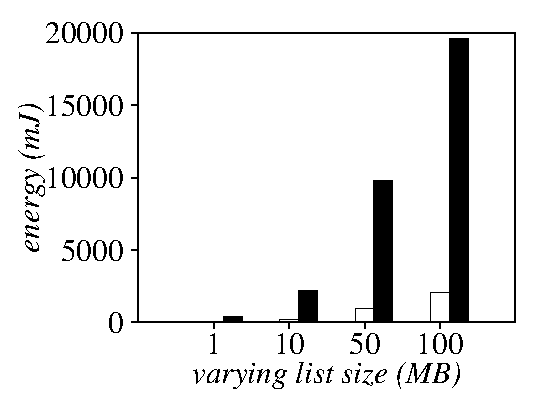
\includegraphics[width=0.5\columnwidth]{figures/Difference-energy-VaryListLen.eps}\\
  (a) query latency & (b) energy
\end{tabular}
  \caption{Varying the list size (for difference)}
  \label{fig:varyListSizeDifference}
 \end{figure}



\textbf{Effect of varying list size skewness factor}.
The skewness factor $f$ is a key parameter in \textsf{difference} operation.
Let $A$ and $B$ be two inverted lists. Unlike the default case, $A$ is not necessarily shorter than $B$. It depends on the skewness factor $f$ (still defined as $|B|/|A|$).
We vary $f$ from 0.01 to 100 (Table~\ref{tab:skewFactorDifference} explains the corresponding sizes of list $A$ and $B$). Thus, $f<1$ means $A$ is longer than $B$. We consider the operation $(A-B)$. Figure~\ref{fig:varyListSkewDifference} plots the effect of skewness factor $f$.

There are several interesting results.
(1) Compared to regular SSD, Smart SSD has a longer query latency when the skewness factor $f=0.01$ and $f=0.1$ (in these two cases, $|A| > |B|$). Assuming the $|A\cap B|$ is very small, the result size of $(A-B)$ is very close to $|A| + |B|$. E.g., when $f=0.01$, $\frac{|A-B|}{|A| + |B|}=98.6\%$. So, if $|A| > |B|$, it is not cost-effective to offload $(A-B)$ because it does not save much data transfer.
(2) Smart SSD, on the other hand, shows better performance when $f\ge 1$ (i.e., $|A| \le |B|$). That is because $|A-B| \le |A| \le (|A| + |B|)/2$. Meaning that offloading $(A-B)$ can save at least 50\% of the data transfer.
(3) For Smart SSD, the query latency increases when $f$ goes from 0.01 to 0.1, but decreases afterward when $f>0.1$. 
We can analyze this as follows. Let $n_1$ and $n_2$ be the number of entries of list $A$ and $B$, when $f=0.01$ or $f=0.1$ ($n_1>n_2$). Then, the estimated number of memory accesses is $n_1\cdot\log n_2$. When $f$ increases from 0.01 to 0.1, $n_2$ increases (but $n_1$ remains the same). Consequently, it incurs more memory accesses. However, when $f=1$, the element checking algorithm is switched to the linear search (see Section~\ref{sec:difference}). Thus, the estimated number of memory accesses is $(n_1 + n_2)$. When $f=10$ or $f=100$ ($n_1<n_2$), the algorithm switches back to the binary search. However, since $n_1<n_2$ when $f>1$, it causes even less memory accesses. Table~\ref{tab:skewFactorDifference} shows the actual number of memory accesses.


%(3) For Smart SSD, the query latency increases when $f$ goes from 0.01 to 0.1, but decreases when $f$ is larger. We explain it as follows. Let $n_1$ and $n_2$ be the number of entries of list $A$ and $B$, when $f=0.01$ or $f=0.1$ ($n_1>n_2$), the estimated number of memory accesses is $n_1\cdot\log n_2$. When $f$ goes from 0.01 to 0.1, $n_2$ increases (but $n_1$ stays the same). Thus, it incurs more memory accesses. However, when $f=1$, the element checking algorithm is switched to linear search (see Section~\ref{sec:difference}). Thus, the estimated number of memory accesses is $(n_1 + n_2)$. When $f=10$ or $f=100$ ($n_1<n_2$), the algorithm is switched back to binary search again. However, $n_1<n_2$ when $f>1$, thus, introducing even less memory accesses. See Table~\ref{tab:skewFactorDifference} for the actual number of memory accesses.
(4) For regular SSD, it shows a similar trend to Smart SSD when $f$ increases. However, when $f$ changes from 0.01 to 1, unlike Smart SSD, its latency still increases because, for regular SSD, I/O time is a dominant factor. In other words, when $f=1$, both $A$ and $B$ are of 10 MB, where the total data size greater than all the other cases.
(5) As a comparison, when $f=1$, both lists are a size of 10 MB. This case is similar to Figure~\ref{fig:varyInterRatioIntersection2}(a) when the intersection ratio is 100\%. Both adopt sort-merge based algorithm, and can save around 50\% of data transfer. Thus, it shows a similar result in~\ref{fig:varyInterRatioIntersection2}(a).
(6) In terms of energy consumption, Smart SSD always achieves better performance with the help of its power-efficient processors inside SSD.

In short, we can deliver the following implication in Figure~\ref{fig:varyListSkewDifference}: \emph{for the \textsf{difference} operation $(A-B)$, Smart SSD can win only if $|A| \le |B|$}.

\begin{figure}[tbp]
  \centering
    \begin{tabular}{ccc}
 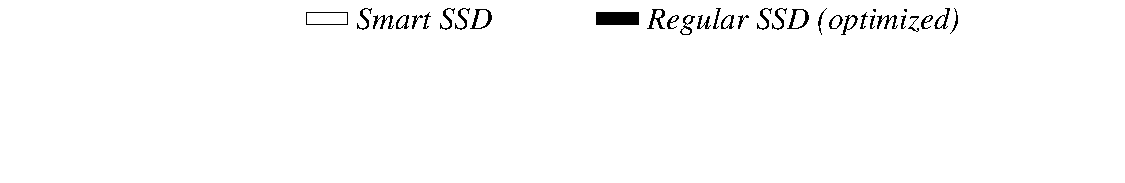
\includegraphics[width=0.52\columnwidth]{figures/banner2.pdf}%banner2.pdf
\end{tabular}
\vspace{-0.1cm}
\renewcommand{\tabcolsep}{0.1mm}


  \begin{tabular}{ccc}
 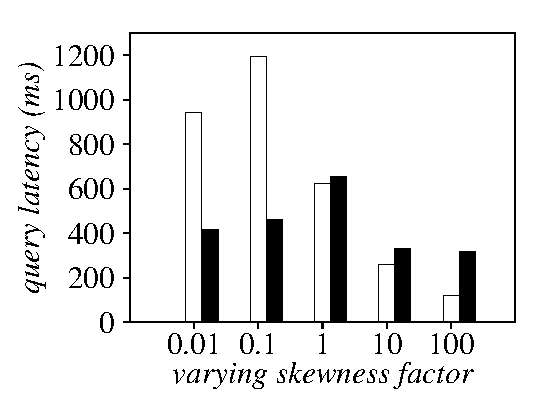
\includegraphics[width=0.5\columnwidth]{figures/Difference-time-VaryListSkew.eps}&
  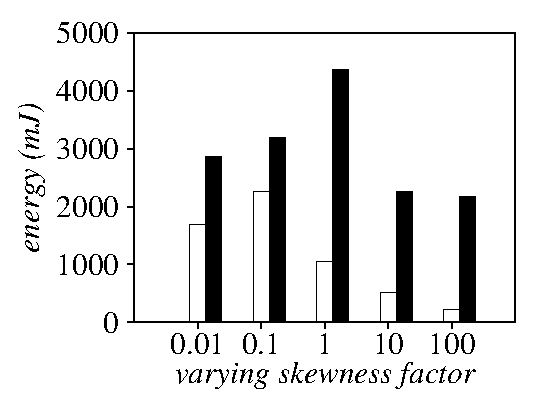
\includegraphics[width=0.5\columnwidth]{figures/Difference-energy-VaryListSkew.eps}\\
  (a) query latency & (b) energy
\end{tabular}

  \caption{Varying the list size skewness factor (for difference)}
  \label{fig:varyListSkewDifference}
 \end{figure}


\begin{table}[tbp]\small
\centering
\begin{tabular}{l|r|r|r}\hline\hline
\textbf{Skewness factor} & \textbf{List $A$ size} & \textbf{List $B$ size} & \textbf{\# of DRAM access}\\\hline
0.01 & 10 MB & 0.1 MB &3,512,670\\\hline
0.1 & 10 MB & 1 MB&4,611,592\\\hline
1 & 10 MB & 10 MB&982,012\\\hline
10 & 1 MB & 10 MB& 581,830\\\hline
100 & 0.1 MB & 10 MB&59,478\\\hline\hline
\end{tabular}
\caption{Corresponding list sizes and number of memory accesses with different skewness factors in Figure~\ref{fig:varyListSkewDifference}}\label{tab:skewFactorDifference}
\end{table}

%\begin{figure}[hbtp]
%  \centering
%    \begin{tabular}{ccc}
% 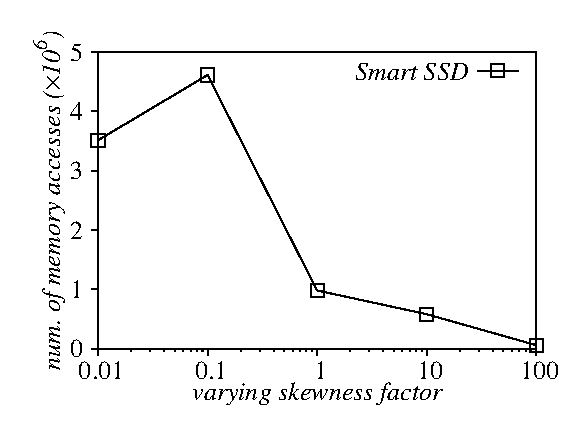
\includegraphics[width=0.6\columnwidth]{figures/Difference-Avg-Mem.eps}
%\end{tabular}
%  \caption{Num of memory access in Figure \ref{fig:varyListSkewDifference}}
%  \label{fig:numMemAccDiff}
% \end{figure}

%1. Smart SSD loses at 0.01 and 0.1 point. at 0.01, A = 10 MB, B = 0.1MB, A-B does not save much, result size is 326437. at 0.1, A = 10MB, B = 1MB, A-B also does not save much, result size is 327790

%2. For Smart SSD, why worse at 0.1? Compare 0.01 and 0.1 points, both A = 10MB, but at 0.1 point, B is large. According to A*log B, meaning that, at 0.1 point, memory access more. Although at 0.1 point, total num of pages are a little more (1412 vs 1290), on avg, 0.1 point, avg mem access per page is higher (3266 vs 2723)

% 3. For Smart SSD, why win at 1 point? as two lists are of 10MB, in which case, save at least one list transfer

% 4. For Smart SSD, why win at 10 and 100? less data transfer

%5. For normal SSD, why it reaches the highest point at 1? as two lists are 10MB, more data transfer

%6. why 10 is less than 0.1? as 10*log (0.1) vs 0.1*log(10)

%7. Comparison: 10MB vs 10MB, i.e, at point skew 1. This case is similar to Fig 9a(100\% point). As, both are saving around one list. And, using sort-merge algo. Echo results!


\textbf{Effect of varying intersection ratio}.
The intersection ratio is also a crucial parameter to $(A-B)$. It determines the result size, which can affect the system performance in two aspects: (1) data transfer cost and (2) ranking cost (at host side). Intuitively, the higher intersection ratio, the smaller result size. We set the size of list $A$ to the same as list $B$ in this case\footnote{\small As discussed before, since there is no noticeable changes when the size of list $A$ is 0.01\% of list $B$, we omit the results.}. As shown in Figure~\ref{fig:varyInterRatioDifference}, for Smart SSD, both the latency and energy consumption generally decreases as the intersection ratio increases, specifically from 10\% to 100\% due to lower data transfer cost and ranking cost. For regular SSD, its performance gain results solely from lower ranking cost. Figure~\ref{fig:varyInterRatioDifference} delivers the following message: \emph{Smart SSD favors lists with a smaller intersection ratio for the \textsf{difference} operation}.

\begin{figure}[tbp]
\centering
\begin{tabular}{ccc}
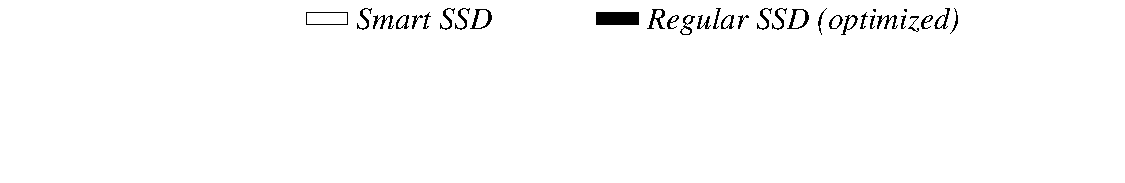
\includegraphics[width=0.52\columnwidth]{figures/banner2.pdf}
\end{tabular}
\vspace{-0.1cm}
\renewcommand{\tabcolsep}{0.1mm}
\begin{tabular}{ccc}
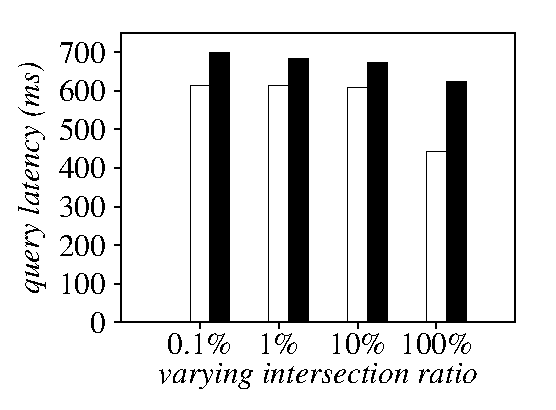
\includegraphics[width=0.5\columnwidth]{figures/Difference-time-VaryInterRatio-equal.eps}&
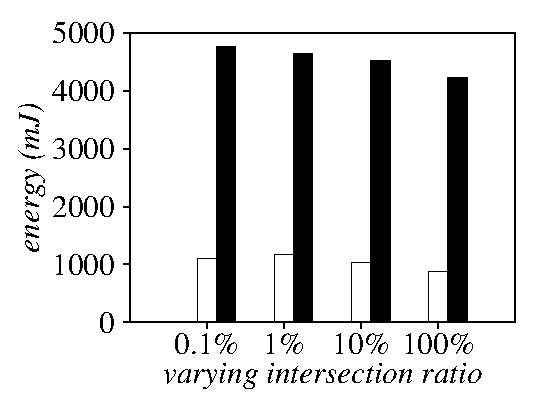
\includegraphics[width=0.5\columnwidth]{figures/Difference-energy-VaryInterRatio-equal.eps}\\
(a) query latency & (b) energy
\end{tabular}
\caption{Varying intersection ratio (for difference)}
\label{fig:varyInterRatioDifference}
\end{figure}

\textbf{Remark}. It is cost-effective to offload the \textsf{difference} operation $(A-B)$ only if $|A| \le |B|$, and Smart SSD favors lists with a smaller intersection ratio.

\subsection{Ranked Difference}\label{sec:expRankedDifference}
We offload the \textsf{ranked difference} (i.e., step S3, S4, and S5 in Figure~\ref{fig:SmartSSDLucene}) to Smart SSD.
As discussed before, compared to the non-ranked operation, offloading the ranked operation can reduce data transfer cost, but increase ranking cost. When the result size is large, Smart SSD can benefit because it can save more data transfer time at the cost of extra ranking overhead. On the other hand, there is no notable performance gain when the result size is small (e.g., less than 30,000 entries).

\textbf{Results on real data}.
The results are similar to non-ranked difference (see Table~\ref{tab:diffRealData}) because the result size is small (3,109 on average).

%See Table~\ref{tab:rankDiffRealData}, which is similar to Table~\ref{tab:diffRealData} as the average result size is small (3109 on average).

%\begin{table}[tbp]\small
%\centering
%\begin{tabular}{l|c|c}\hline\hline
%& \textbf{Query latency (ms)} & \textbf{Energy (mJ)}\\\hline
%Smart SSD & 77  & 139\\\hline
%Regular SSD & 168 & 1109 \\\hline\hline
%\end{tabular}
%\caption{Ranked difference on real data \textcolor{red}{omit}}\label{tab:rankDiffRealData}
%\end{table}

\textbf{Effect of varying list size}.
Similar to non-ranked version (please see Figure~\ref{fig:varyListSizeDifference}) as the result size is small (maximum is 32,204).

\textbf{Effect of varying list size skewness factor}.
The skewness factor determines the result size. For the non-ranked Difference (please refer to Figure~\ref{fig:varyListSkewDifference}),
Smart SSD has a longer query latency when $f=0.01$ and $f=0.1$ due to the large result size. Thus, if ranking function is applied, the result size will be much smaller. Therefore, we can expect Smart SSD achieves better performance (i.e., shorter latency) than the regular SSD in all cases.

However, surprisingly, Smart SSD still has a longer query latency than the regular SSD when $f=0.01$ and 0.1.
That is because the ranking function is applied only when all the results are available by the \textsf{difference} operation.
This requires too many memory accesses to return the results (as analyzed in Section~\ref{sec:expDifference}) regardless of any data transfer. The situation could be changed if we combine both ranking and difference together by adopting a top-$k$ ranking algorithm \cite{Fagin2001, Broder2003EQE}.

It is also interesting to see the performance gap (in query latency) between Smart SSD and regular SSD in both Figure~\ref{fig:varyListSkewRankDifference}and Figure~\ref{fig:varyListSkewDifference} when $f=1$. For Smart SSD, query latency in ranked difference is faster than that in non-ranked difference, which comes from less data transfer.

\begin{figure}[tbp]
  \centering
    \begin{tabular}{ccc}
 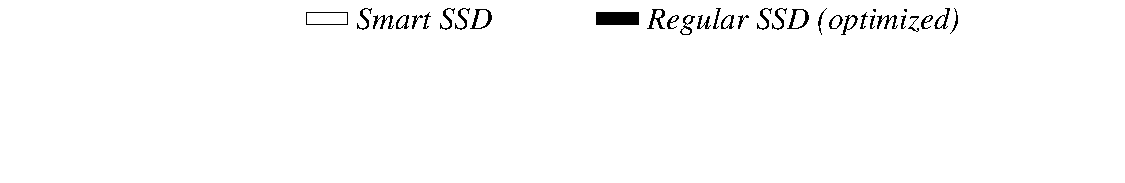
\includegraphics[width=0.52\columnwidth]{figures/banner2.pdf}%banner2.pdf
\end{tabular}
\vspace{-0.1cm}
\renewcommand{\tabcolsep}{0.1mm}


  \begin{tabular}{ccc}
 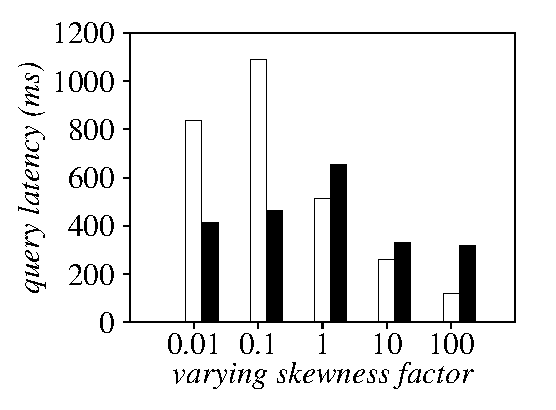
\includegraphics[width=0.5\columnwidth]{figures/RankDifference-time-VaryListSkew.eps}&
  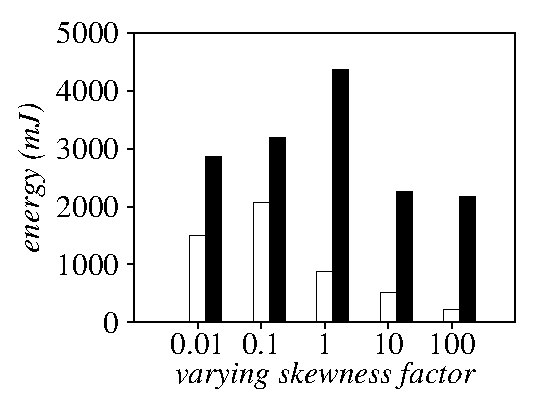
\includegraphics[width=0.5\columnwidth]{figures/RankDifference-energy-VaryListSkew.eps}\\
  (a) query latency & (b) energy
\end{tabular}

  \caption{Varying the list size skewness factor (for ranked difference)}
  \label{fig:varyListSkewRankDifference}
 \end{figure}

%\textcolor{red}{Exp: should be different from non-ranked version. We will always win.} However, we lose! That is because the memory access it too many (in order to get the results)

%1. At 100 and 10, we win

%2. Why lose at 0.01 and 0.1? That's because in order to get the intersection results, we accessed too many memory! A*logB.

%3. Why still win at 1? (1) mem access is small as using sort-merge; (2) the gap is larger, as no need for data transfer.
% (3) save one list transfer. Actually, similar to Fig11a: Comparison: 10MB vs 10MB, i.e, at point skew 1.
% This case is similar to Fig11a(100\% point). As, both are saving around one list. And, using sort-merge algo.
% Echo results!

\textbf{Effect of varying intersection ratio}.
Figure~\ref{fig:varyInterRatioRankDifference} shows the impact of varying intersection ratio to system performance.
It clearly shows the superiority of Smart SSD in terms of both query latency and energy consumption. Compared to Figure~\ref{fig:varyInterRatioDifference}, the performance gap between Smart SSD and regular SSD is larger in terms of different intersection ratios. That is because of less data transfer after ranking.
 \begin{figure}[tbp]
\centering
\begin{tabular}{ccc}
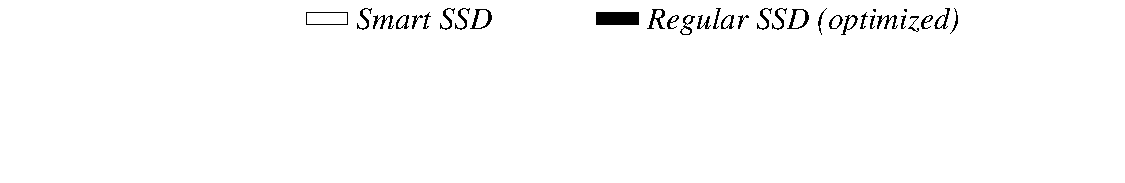
\includegraphics[width=0.52\columnwidth]{figures/banner2.pdf}
\end{tabular}
\vspace{-0.1cm}
\renewcommand{\tabcolsep}{0.1mm}
\begin{tabular}{ccc}
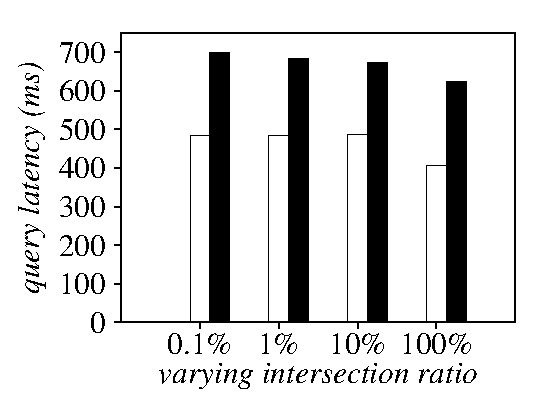
\includegraphics[width=0.5\columnwidth]{figures/RankDifference-time-VaryInterRatio-equal.eps}&
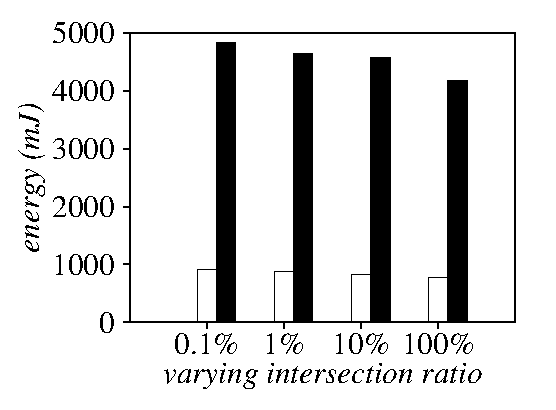
\includegraphics[width=0.5\columnwidth]{figures/RankDifference-energy-VaryInterRatio-equal.eps}\\
(a) query latency & (b) energy
\end{tabular}
\caption{Varying intersection ratio (for ranked difference)}
\label{fig:varyInterRatioRankDifference}
\end{figure}


\subsection{Ranked Union}\label{sec:expRankedUnion}
In this case, we offload the \textsf{ranked union} (i.e., step S3, S4, and S5 in Figure~\ref{fig:SmartSSDLucene}) to Smart SSD. We first present the results in Section~\ref{sec:rankUnionResults}, then discuss more on optimizations in Section~\ref{sec:rankUnionOpt}.

\subsubsection{Results}\label{sec:rankUnionResults}
\textbf{Results on real data}.
Table~\ref{tab:unionRealData} shows the experimental results with real data: Smart SSD is slower around 1.7$\times$ compared to regular SSD in query latency. That is due to too many memory accesses. As discussed in Section~\ref{sec:union}, every list has to be scanned around $2u$ times, where $u$ is the number of lists in a query. On average, $u=3.8$ in our query log. However, Smart SSD still can benefit from energy consumption by 2.1$\times$ with the help of its power-efficient processors.


\begin{table}[tbp]\small
\centering
\begin{tabular}{l|c|c}\hline\hline
& \textbf{Query latency (ms)} & \textbf{Energy (mJ)}\\\hline
Smart SSD & 505 & 960 \\\hline
Regular SSD & 299 & 2033  \\\hline\hline
\end{tabular}
\caption{Ranked union on real data}\label{tab:unionRealData}
\end{table}

We omit the results of varying intersection ratios, list size skewness factors, and list sizes, for space constrains. The short summary of the results is as follows; Smart SSD is slower around 1.2$\times$ in query latency, but saves energy around 2.8$\times$. Next, we explore the effect of varying number of lists, which is a key parameter.

%\textbf{Effect of varying intersection ratio}.
%The intersection ratio determines the result size.
%Figure~\ref{fig:varyInterRatioRankUnion} evaluates the impact of intersection ratio to system performance, with two equal-sized lists (10 MB).
%It shows, except when the intersection ratio is 100\%, Smart SSD loses around 1.2$\times$ in query latency. That is because, the result size is smaller than other cases, incurring less number of memory accesses.
%
%\begin{figure}[tbp]
%\centering
%\begin{tabular}{ccc}
%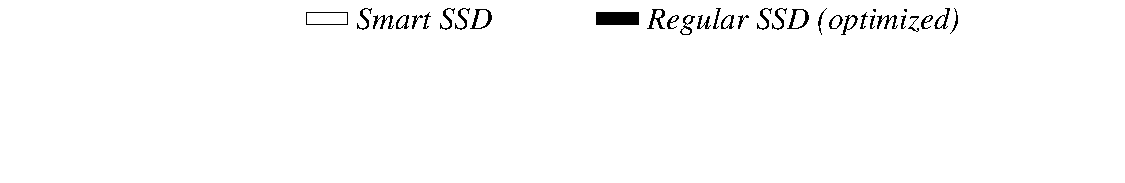
\includegraphics[width=0.52\columnwidth]{figures/banner2.pdf}
%\end{tabular}
%\vspace{-0.1cm}
%\renewcommand{\tabcolsep}{0.1mm}
%\begin{tabular}{ccc}
%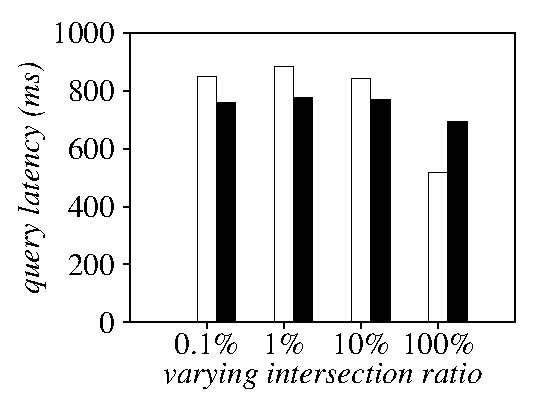
\includegraphics[width=0.5\columnwidth]{figures/RankUnion-time-VaryInterRatio.eps}&
%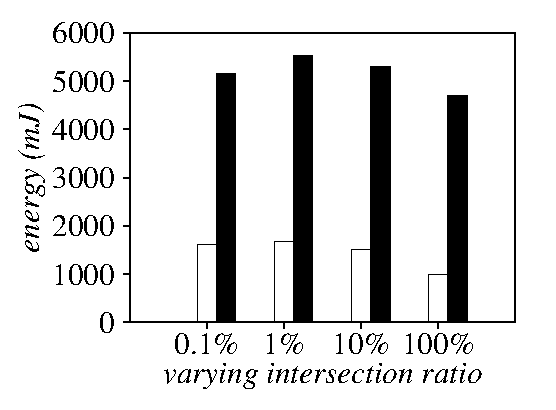
\includegraphics[width=0.5\columnwidth]{figures/RankUnion-energy-VaryInterRatio.eps}\\
%(a) query latency & (b) energy
%\end{tabular}
%\caption{Varying intersection ratio (for ranked union)}
%\label{fig:varyInterRatioRankUnion}
%\end{figure}
%
%
%\textbf{Effect of varying list size skewness factor}.
%Figure~\ref{fig:varyListSkewRankUnion} shows the impact of the skewness factor. In all cases, Smart SSD loses around 1.2$\times$.
%
%\begin{figure}[tbp]
%  \centering
%    \begin{tabular}{ccc}
% 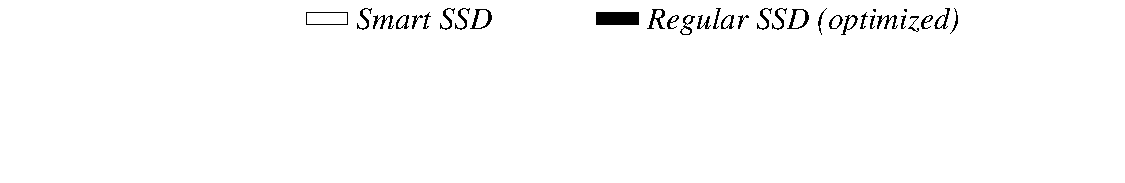
\includegraphics[width=0.52\columnwidth]{figures/banner2.pdf}%banner2.pdf
%\end{tabular}
%\vspace{-0.1cm}
%\renewcommand{\tabcolsep}{0.1mm}
%
%
%  \begin{tabular}{ccc}
% 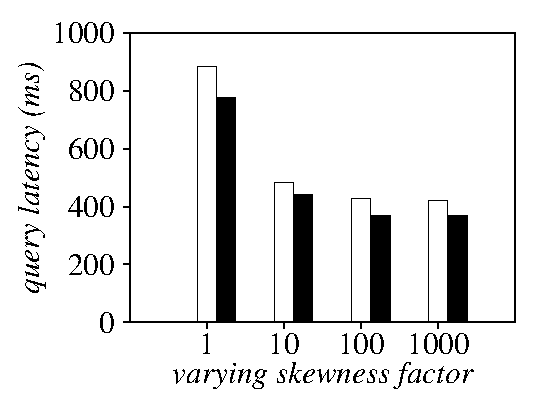
\includegraphics[width=0.5\columnwidth]{figures/RankUnion-time-VaryListSkew.eps}&
%  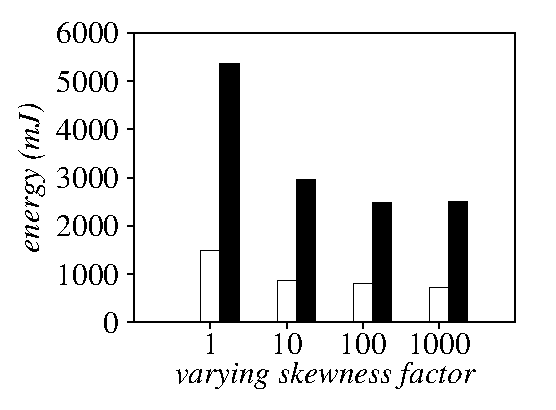
\includegraphics[width=0.5\columnwidth]{figures/RankUnion-energy-VaryListSkew.eps}\\
%  (a) query latency & (b) energy
%\end{tabular}
%
%  \caption{Varying the list size skewness factor (for ranked union)}
%  \label{fig:varyListSkewRankUnion}
% \end{figure}
%
%
%\textbf{Effect of varying list size}.
%Figure~\ref{fig:varyListLenRankUnion} shows the impact of list size. In all cases, Smart SSD loses around 1.2$\times$.
%
%  \begin{figure}[tbp]
%  \centering
%    \begin{tabular}{ccc}
% 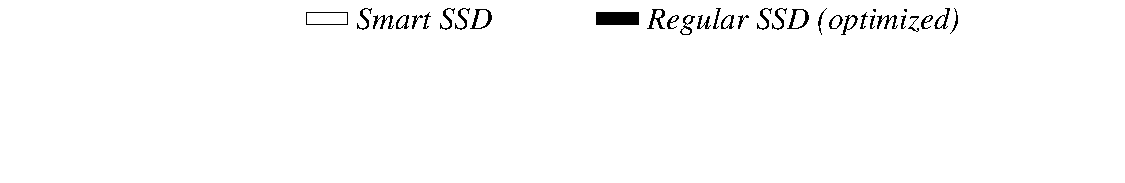
\includegraphics[width=0.52\columnwidth]{figures/banner2.pdf}
%\end{tabular}
%\vspace{-0.1cm}
%\renewcommand{\tabcolsep}{0.1mm}
%  \begin{tabular}{ccc}
% 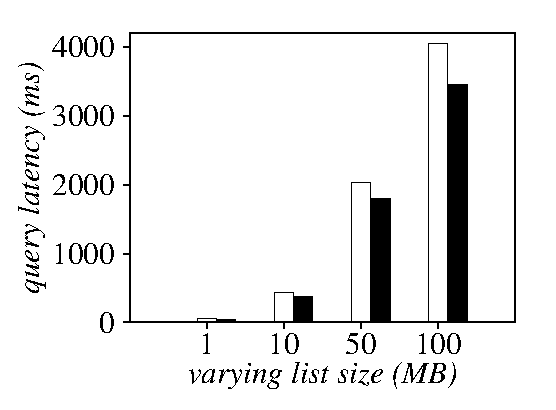
\includegraphics[width=0.5\columnwidth]{figures/RankUnion-time-VaryListLen.eps}&
%  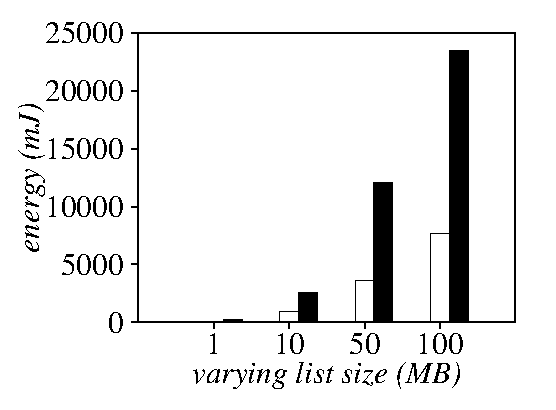
\includegraphics[width=0.5\columnwidth]{figures/RankUnion-energy-VaryListLen.eps}\\
%  (a) query latency & (b) energy
%\end{tabular}
%  \caption{Varying the list size (for ranked union)}
%  \label{fig:varyListLenRankUnion}
% \end{figure}
%


\textbf{Effect of varying number of lists}
Figure~\ref{fig:varyNumKeywordsRankUnion} displays the impact of number of lists $u$ in a query. The query latency gap between Smart SSD and regular SSD gets larger with more number of lists. That is because each list has to be accessed approximately $2u$ times.
  \begin{figure}[tbp]
  \centering
    \begin{tabular}{ccc}
 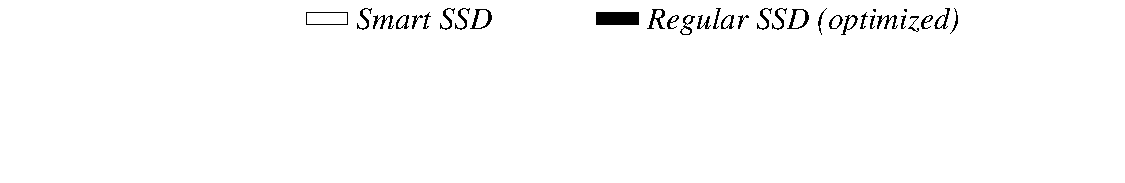
\includegraphics[width=0.52\columnwidth]{figures/banner2.pdf}
\end{tabular}
\vspace{-0.1cm}
\renewcommand{\tabcolsep}{0.1mm}
  \begin{tabular}{ccc}
 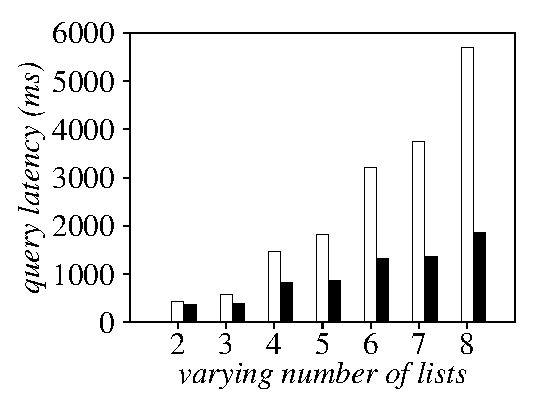
\includegraphics[width=0.5\columnwidth]{figures/RankUnion-time-VaryNumLists.eps}&
  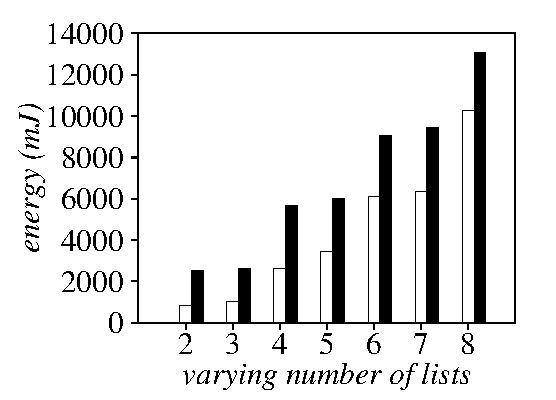
\includegraphics[width=0.5\columnwidth]{figures/RankUnion-energy-VaryNumLists.eps}\\
  (a) query latency & (b) energy
\end{tabular}
  \caption{Varying the number of lists (for ranked union)}
  \label{fig:varyNumKeywordsRankUnion}
 \end{figure}


\subsubsection{Discussion: Call for Algorithmic Optimizations}\label{sec:rankUnionOpt}
Because of too many memory accesses, it is not cost-effective to offload ranked union to Smart SSD.
To resolve this limitation, on the one hand, we fundamentally need to improve the innate memory access speed of Smart SSD through its hardware upgrade. On the other hand, more efficient algorithms could be designed to reduce memory access. Our current implementation (following Lucene) solves the ranking problem when all the union results are available, then scores every qualified document. However, both union and ranking could be algorithmically combined for early termination~\cite{Broder2003EQE,Fagin2001}. This means we do not need to scan all the union results. We will explore the early pruning techniques in the future work.

%Because of too many memory accesses, it is not cost-effective to offload ranked union to Smart SSD. To resolve this limitation, on the one hand, we fundamentally need to improve the innate memory access speed of Smart SSD through its hardware update. On the other hand, more efficient algorithms could be designed to reduce memory access. Our current implementation (following Lucene) solves the ranking problem when all the union results are available, then scores every qualified document. However, union and ranking could be algorithmically combined for early termination~\cite{Broder2003EQE,Fagin2001}. Meaning that, we do not need to scan all the union results. We will explore the early pruning techniques in the future work.


%More importantly, one needs to be careful about the \emph{hidden constant} of algorithms, not only big O notation. E.g., the sort-merge based union algorithm is in linear cost, however, the hidden constant factor slows down the performance significantly.



%\textbf{Algorithmically combined (may be a possible)\cite{topk}.}

%\textbf{A special case of ranked union on \emph{two} lists.} If the number of lists is 2, a better algorithm for Smart SSD can be as follows. (1) Find the intersection results $R$ between $k$ lists $L_1, L_2, \cdots, L_k$. It takes, usually, less than 1 scan of all lists; (2) Scan Scan $R$, and $L_1, L_2, \cdots, L_k$ to find the top ranked results. It takes 1 scan. Thus, in total, around 2 full scans on all the $k$ lists. In this case, Samrt SSD wins. 